\chapter{Optimierung der Verstärkung eines Triple GEM Detektors}

	\section{Aufbau des Detektors}
		\subsection{Detektorkonfiguration}
	Die systematische Erfassung von Verstärkung und Energieauflösung erfordert eine Detektoranordnung, die die flexible Variation der Felder ermöglicht und vergleichsweise einfach zu unterhalten ist. Zu diesem Zwecke wird die Konfiguration aus Abbildung \ref{fig:Konzeptskizze GEM Aufbau} in einem eigens für solche Zwecke konzipierten Detektor gebaut \cite{DetektorPrototyp}. \\
	\\
	 Hierzu werden die GEM-Folien auf Rahmen gespannt, die es ermöglichen die Folien in eine dafür vorgesehene Halterung einzusetzen (siehe Abbildung \ref{fig:CAD-Zeichnung}), der Abstand der einzelnen Folien und Platten kann variabel über Abstandsbolzen eingestellt werden. Die Rahmenanordung wird dann in dem Aluminiumgehäuse fixiert. Das Alumniniumgehäuse bietet dabei Anschlüsse für die Hochspannungskabel zum Betrieb des Detektors, sowie Anschlüsse zur Auslese der Messereignisse und Anschlüsse für Gaszu- und Abfluss. Die Strahlung kann durch dafür vorgesehene Fenster eingestrahlt werden, die auf dem Aluminumverdeck und an der Seite sind. Für den Fall der Einstrahlung von oben wurde die Driftfeldanode in zwei Anoden aufgeteilt, da so Elektronen-Ionen-Paare, die über der Driftkammer entstehen von der oberen Platte abgefangen werden können und so keine Schwankungen im Driftfeld zulässt. Auf diese Weise wird der Detektor sicherer gegen Störeinflüsse geschützt.
	 \begin{figure}[h]
	 	\centering
	 	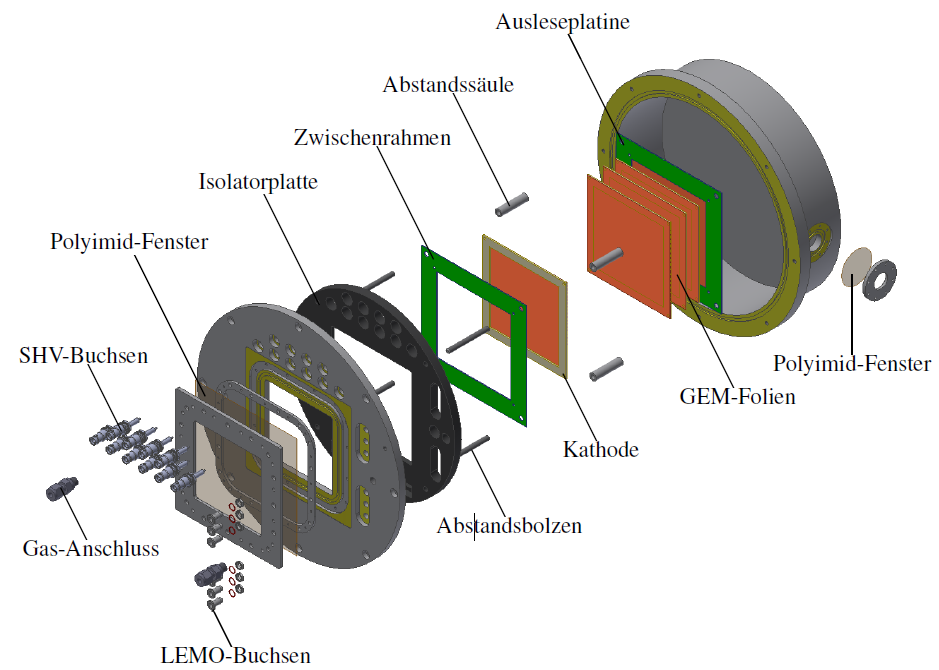
\includegraphics[scale=0.45]{CAD-Zeichnung.png}
	 	\caption{CAD-Zeichnung des Detektors bestehend aus den einzelnen Anschlüssen und der Rahmenstruktur zum Befestigen der einzelnen GEM-Folien, entnommen aus \cite{ottnad}}
	 	\label{fig:CAD-Zeichnung}
	 \end{figure}

\newpage


		\subsection{Auslese- und Betriebselektronik}
		In diesem Absatz sollen die Grundlagen der verwendeten Elektronik beschrieben und begründet werden. In Abbildung \textcolor{blue}{Blockschaltbild von Betriebs und Ausleseelektronik}. ist das Konzeptionelle Blockschaltbild zu sehen, mit dem die Messungen stattfinden. Die GEM-Folien werden über einen Hochspannungsgenerator des Modells betrieben, wobei ein Pikoamperemeter des Typs \textcolor{red}{Zagreb-Pikoampermeter-Ident} davorgeschaltet wird. Dies ermöglicht die Detektion von Gasentladungen, durch die kurzweilige aber vergleichsweise große Ströme entstehen können, wobei dann Schritte ergriffen werden können, um die Detektoranordnung vor großflächigeren Schäden zu schützen. Die Spannungen sind über eine zentralisierte Slow-Control steuerbar und können anwendungsbedingt auf eine Genauigkeit von einem Volt \textcolor{red}{Verifikation} eingestellt werden. \textcolor{red}{gehe auf die Süezifikationen der Schaltung ein, siehe Ottnad Arbeit} \\
		\\
		Die Ausleseanordnung besteht aus einem Vorverstärker des Modells \textcolor{red}{Modelltyp und Verstärkung} und einem Impulsformenden Verstärker des Modells \textcolor{red}{Modelltyp}. Hier sind die Verstärkung und die Signalformzeit aus gegebenen Einstellungen wählbar. Das geformte und Verstärkte Signal wird dann auf einen Vielkanalzähler gegeben, welcher die einkommenden Signale auf einzelne Bins je nach Amplitude verteilt. Das resultierende MCA-Spektrum kann dann entweder durch die Slow-Control oder ein dafür vom Hersteller vorgesehenes Programm aufgenommen werden.\\
		Alternativ kann die Auslese auch direkt an einen anderen Kanal des Pikoamperemeters angeschlossen werden, um den in der Messelektonik induzierten Strom zu bestimmen. Es ergibt sich ein Blockschaltbild wie in Abbildung \textcolor{red}{Blockschaltbild II}  
		
		\subsection{Gasqualitätssicherung und Druck-Temperatur-Überwachung}
		Neben einer starken Feldabhängigkeit ist die effektive Verstärkung in einem GEM-Detektor auch abhängig von dem Druck und der Temperatur des aktiven Mediums. Da das System nicht komplett isolierbar ist, müssen Druck und Temperaturschwankungen entsprechend überwacht und deren Einfluss aus den Messergebnissen rausgerechnet werden. Insbesondere sind Unreinheiten im Gas nicht gewünscht, sodass auch die Verunreinigungen des Gases überwacht werden müssen.\\
		\\
		Zum Überwachen der Druck- und Temperaturschwankungen wird dazu ein Laborlogger verwendet. Hierbei wird ein Sensor der Klasse MS5611 verwendet, der Prinzipiell im Stande dazu ist Druck, Temperatur und Luftfeuchte zu messen \cite{LoggerSensor}. Die Genauigkeit der Druckmessung liegt dabei  bei $\pm 1.5 \si{mbar}$  ; die Genauigkeit der Temperaturmessung liegt bei $\pm 0.8 \si{^\circ C}$. Der Sensor wird über einen Microcontroller des Typs \textcolor{red}{Typ Microcontroller} ausgelesen und die Daten werden an eine Datenbank übergeben \cite{Hauer}.\\
		Die Reinheit des Gases wird durch einen Vielgasanalysator des Modells \textcolor{red}{Rapidoxmodell} überwacht. Hierbei werden Sauerstoff- und Wassergehalt gemessen. 
		

	\section{Messmethodik}
		\subsection{Über die Eignung von $\ce{^{55}}$Fe-Isotopen}\label{sec:Fe55}
			Die Untersuchung der Effekte der einzelnen Felder eines Triple-GEM-Detektors auf seine Energieauflösung und Verstärkung erfordert eine fundierte Kenntnis der zur Messung verwendeten Strahlung. Eine geeignete Strahlenquelle muss daher einige Anforderungen erfüllen, um den Optimierungsprozess zu ermöglichen. Die Eignung einer  $\ce{^55Fe}$ Quelle kann dabei wie folgt begründet werden:\\
			\\
			Das Isotop $\ce{^55Fe}$ zerfällt durch Elektronen-Einfang zu Mangan, welches durch Emission von Röntgenstrahlung in seinen Grundzustand übergeht, das resultierende Mangan-Isotop $\ce{^55 Mn}$ ist stabil. Mit einer Halbwertszeit von 2,75 Jahren \cite{Half_Life_FE55} gewährleistet die Quelle während des gesamten Optimierungsprozesses eine konstante Strahlleistung und so einen stabilen Energiepegel. Insbesondere sind Verzerrungen durch Sekundärzerfälle ausgeschlossen.\\
			Das Spektrum wird hauptsächlich von den $K_{\alpha}$- und $K_{\beta}$-Linien dominiert, was sicherstellt, dass die gesamte Energie im System deponiert wird (siehe Kapitel \ref{chap:Photonen}). Dadurch werden statistische Unsicherheiten in der Energiedeposition und damit verbundene Einflüsse auf die Energieauflösung minimiert. Eine Sammlung der relevanten Eisenlinien findet sich in Tabelle \ref{tab:Eisenlinien}.
			
			\begin{table}[h!]
				\centering
				\begin{tabular}{|l|c|c|}
					\hline
					\textbf{Linie} & \textbf{Energie / keV} & \textbf{Rel. Intensität} \\ \hline
					K\textsubscript{$\alpha$}-Photo 1    & 5,755         & 0,540           \\ \hline
					K\textsubscript{$\alpha$}-Photo 2    & 5,716         & 0,117           \\ \hline
					K\textsubscript{$\alpha$}-Photo 3    & 5,815         & 0,078           \\ \hline
					\textbf{K\textsubscript{$\alpha$}-Photo}  & 5,755         & 0,777           \\ \hline
					\textbf{K\textsubscript{$\alpha$}-Escape} & 2,892         & 0,121           \\ \hline
					K\textsubscript{$\beta$}-Photo 1     & 6,351         & 0,061           \\ \hline
					K\textsubscript{$\beta$}-Photo 2     & 6,312         & 0,013           \\ \hline
					K\textsubscript{$\beta$}-Photo 3     & 6,411         & 0,009           \\ \hline
					\textbf{K\textsubscript{$\beta$}-Photo}  & 6,351         & 0,088           \\ \hline
					\textbf{K\textsubscript{$\beta$}-Escape} & 3,488         & 0,014           \\ \hline
				\end{tabular}
				\caption{relevante Linien des Eisenspektrums einer $\ce{^55 Fe}$-Quelle in Argon, entnommen aus \cite{ottnad}. Hervorgehoben sind die Linien, die das Signal dominieren}
				\label{tab:Eisenlinien}
			\end{table}
			
			
			\noindent Die im Optimalfall erreichbare Energieauflösung überschreitet die Energieabstände der einzelnen $K$ Linien. Diese Aussage trifft sowohl für den Photopeak, als auch für den Escape-Peak zu, sodass diese offenbar nicht eindeutig auflösbar sind. Entsprechend müssen nur wesentliche Linien berücksichtigt werden
			
			
			
			 Die Bestimmung der Detektorparameter stützt sich auf die Bestimmung der Parameter des Photopeaks, es wird demnach das Spektrum angepasst, das aufgrund der Nähe der Linien vollumfänglich durch folgende Funktion beschrieben werden kann \cite{Hauer}. für die folgende Diskussion, sollen die einzelnen Signalteile entsprechend ihrer Bedeutung diskutiert werden.
			 

			\begin{enumerate}
				\item \textbf{Photopeak} Der Photopeak setzt sich aus den Photopeaks für $\text{K}_{\alpha}$- und $\text{K}_{\beta}$-Linie zusammen. Um die Zahl der freien Parameter des Modells zu verkleinern nutzen wir, dass die relativen Intensitäten zu einem Skalierungsfaktor von $8,83$ führen:
				\begin{equation*}
					{ I_{\text{ph}}= A_{{\alpha}} \qty(\exp(\frac{1}{2}\qty(\frac{x-\mu_{{\alpha}}}{\sigma_{\alpha}})^{2})+ \frac{1}{8,8}\exp(\frac{1}{2}\qty(\frac{x-\mu_{{\beta}}}{\sigma_{{\beta}}})^{2}))}
				\end{equation*}
				
				\item \textbf{Escapepeak} Der Escape-Peak wird ein analoger Fit durchgeführt:
				\begin{equation*}
					{    I_{\text{esc}}= A_{{\alpha}}^{\text{Esc}} \qty(\exp(\frac{1}{2}\qty(\frac{x-\mu_{{\alpha}}^{\text{Esc}}}{\sigma_{\alpha}^{\text{Esc}}})^{2})+ \frac{1}{8,8}\exp(\frac{1}{2}\qty(\frac{x-\mu_{{\beta}}^{\text{Esc}}}{\sigma_{{\beta}}^{\text{Esc}}})^{2}))}
				\end{equation*}
				
				\item \textbf{Exponentieller Offset} Es gibt einen Beitrag durch elektronisches Rauschen und durch niederenergetische Fluoreszenz.  Um für diese Effekte zu accounten, schieben wir einen Offset der folgenden Form ein:
				\begin{equation*}
					I_{\text{Off}}= A_{\text{off}} e^{-\frac{x}{c_{\text{char}}}}
				\end{equation*}
				
				\item \textbf{Errorfunction} Auch hier zählen wir das Elektronische Rauschen zu und berücksichtigen, dass das Rauschen am MCA irgendwann nicht mehr zu den Spektren beitragen kann, da kein Signal vorliegt, dass zu einer Signalamplitude in der jeweiligen Range sorgt (quasi Diskriminatorrauschen).
				\begin{equation*}
					I_{\text{erf}}= A_{\text{erf}} \qty(\erf\qty(\frac{x-\mu_{\alpha}}{\sigma_{\alpha}})-1)
				\end{equation*}
			\end{enumerate}
			
			
			
		\subsection{Experimentelle Bestimmung der Verstärkung} \label{sec:Verstärkungsbestimmung}
		Die Bestimmung der Verstärkung wird im folgenden auf zwei Unterschiedliche Wege durchgeführt. Die Methoden sind hierbei auf ihren jeweiligen Zweck, nämlich der quantitativeren oder qualttativeren Verstärkungsbestimmung zugeschnitten.\\
		Die qualtitative Bestimmung der Verstärkung nutzt aus, dass der MCA die Zuordnung zu seinen Bins proportional zur Amplitude des eintreffenden Signals durchführt. Nimmt man für die einzelnen Feldeinstellungen dann ein Spektrum auf, und passt eine Funktion nach Gleichung [REFERENZ] an, dann kann der Peakschwerpunkt des Photopeaks als Funktion der Felder als Proxy für die Verstärkung gewählt werden. Wandert der Schwerpunkt zu höheren Bins, sind die Signalampltiduden offenbar größer und die Signale wurden vorher stärker Verstärkt. Eine solche Methode ist offenbar nur dann sinntragend, wenn es eine Referenz gibt, zu der die Verstärkung relativ untersucht werden kann es handelt sich daher um eine qualitiative Messmethode.\\
		\\
		Quantitativ kann die Verstärkung aus einer Messung des Spektrums und einer Messung des an der Ausleseelektronik induzierten Stromes bestimmt werden. Dazu kann die Auslese des Detektors mit einem Picoamperemeter (MODELL) verbunden werden, sodass die Influenzierten Ströme gemessen werden. In einer darauffolgenden Messung muss dann in derselben Einstellung ein Spektrum gemessen werden; eine parallele Messung ist nicht möglich, da Rauscherscheinungen, die mit den Bauteilen einhergehen einen sehr erheblichen Störeinfluss implizieren, der die Messung nahezu unbrauchbar macht.\\
		Da die Linien der Eisenquelle [ABSCHNITT] hinreichend bekannt sind, können die Linien für eine Energiekalibrierung des MCA für eine gegebene Detektorkonfiguration durchgeführt werden. Damit wird das mit dem MCA gemessene Spektrum zu einem Energie-Histogramm gegebener Bin-weite. Summiert man die einzelnen Ereigniszahlen, gewichtet mit den Energien des jeweiligen Bins auf, erhält man eine Approximation für die im Detektor deponierte Energie und so, unter Berücksichtigung der mittleren Ionisationsenergie (Tabelle \ref{tab:Ionisationsenergien}) eine Näherung für den primären Ionisationsstrom, sofern man die Messdauer berücksichtigt. Die Verstärkung ergibt sich dann entsprechend über den folgenden Zusammenhang:  
		\begin{equation*}
			G=\frac{I_{\text{Readout}}}{I_{\text{Ion}}}
		\end{equation*}
		Es ist offenbar so, dass die quantitative Messung 
		\newpage
	
	\section{Optimierungsmethodik}
	Um eine Optimierung durchführen zu können, wird zunächst eine Referenzmessung durchgeführt. Die aus \cite{ottnad} folgenden Feldeinstellungen (siehe Tabelle \textcolor{red}{Feldertabelle}) werden getestet, um eine für das verwendete Detektorsetup spezifische Vergleichsgröße bestimmen zu können. Diese Referenzgrößen bieten dann die Eckdaten, die die Grundlage des Optimierungsprozesses darstellen.\\
	Der eigentlichen Optimierung wird dann eine Reihe von Analysemessungen vorgeschaltet. Das Ziel dieser Analyse ist es herauszufinden, ob es ein Operationsoptimum im Hinblick auf die Transfereffizienzen gibt, welches es erlaubt die Zahl der für die Optimierung günstigen Detektorkonfigurationen zu reduzieren. Sofern Bedarf besteht, können Einstellungen größerer Verstärkung als Interimskonfigurationen verwendet werden, sofern sie stabile und effiziente Messungen erlauben. Die Analysemessungen sind demnach als iterativer Prozess durchzuführen.\\
	\\
	Um aus den Ergebnissen nun auf potentiell interessante Feldkonfigurationen zu schließen können die Ergebnisse der Analyse verwendet werden, um die Gesamtheit aller Felder aufeinander abzustimmen. Dieses Verfahren soll dabei sicherstellen, dass sowohl die Energieauflösung, als auch die effektive Verstärkung vergleichbar mit den Referenzparametern sind 
	
	\section{Referenzbestimmung}
		\subsection{Methode}
		Über die zentrale Steuerungeinheit lassen sich Feldkonfigurationen vergleichsweise einfach eintragen. In einem ersten Schritt werden daher die Feldeinstellungen aus \cite{ottnad} untersucht, um sicherzustellen, dass die simulierten Ergebnisse mit den Ergebnissen des COMPASS-Experimentes übereinstimmen. In diesem Zusammenhang lassen sich dann die Vergleichsparameter für die Energieauflösung und die effektive Gain bestimmen. Die Einstellungen der Feldkonfigurationen sind in Tabelle \ref{tab:RefKonfig}
		\begin{table}[h!]
			\centering
			\begin{tabular}{|c|c|c|}
				\hline
				&COMPASS & Simulation \\
				\hline
				$E_{\text{D}}\ / \ \ \si{V/cm}$ & 2490 & 2490\\
				\hline
				$U_{\text{GEM}\ 1}/\ \ V$ & 410 & 406  \\
				\hline
				$E_{\text{TF}1} /\ \ \si{V/cm}$ & 3730 & 1753 \\
				\hline
				$U_{\text{GEM}\ 2}/\ \ V$ & 374 & 367  \\
				\hline
				$E_{\text{TF}2} /\ \ \si{V/cm}$ & 3730 & 1578 \\
				\hline
				$U_{\text{GEM}\ 3}/\ \ V$ & 328 & 322  \\
				\hline
				$E_{\text{ind}}/\ \ \si{V/cm}$ & 3730 & 3730  \\
				\hline
			\end{tabular}
			\caption{Sammlung der Detektorfeldkonfigurationen basierend auf den Einstellungen des COMPASS-Experiment und der Ergebnisse der Simulationsergebnisse. Die Originaleinstellungen aus \cite{ottnad} wurden auf die verwendete Gasmischung reskaliert}
			\label{tab:RefKonfig}
		\end{table}
		
		
		
		\noindent Um sicherzustellen, dass die Vergleichsmessungen für beide Einstellungen vergleichbar sind, muss zunächst eine Verstärkerkonfiguration bestimmt werden, die beide Konfigurationen auf dem MCA hinreichend gut auflöst, um sicherzustellen, dass der Anpassungsprozess für beide Spektren funktioniert. Die Messung der Verstärkung wird dann nach dem in Abschnitt \ref{sec:Verstärkungsbestimmung} Verfahren durchgeführt.
		
		\subsection{Ergebnisse}
		
	
	
	
	\newpage
	\section{Parameterscans für die einzelnen Felder}
		\subsection{Untersuchung der Wirkung der Felder auf die Transfereffizienzen}
		
		\subsection{Bestimmung der Auswahlintervalle}
	
	
	\newpage
	\section{Konstruktion und Überprüfung interessanter Detektorkonfigurationen}


\newpage
\chapter{Optimierung der Energieauflösung eines Triple-GEM-Detektors}
	\section{Messmethodik}
	
	\section{Optimierungsmethodik}
	
	\section{Parameterscans für die einzelnen Felder}
	
	\section{Konstruktion und Überprüfung interessanter Detektorkonfigurationen}
	
	
\chapter{Bestimmung des Operations-Optimums}
	\section{Konstruktion von Feldkonfigurationen unter Berücksichtigung von Auflösung und Verstärkung}
	
	\section{Experimentelle Analyse der Konstruierten Konfigurationen}
	
\chapter{Zusammenfassung und Ausblick}
	\section{Zusammenfassung}
	
	\section{Ausblick: Optimierung auf Orts- und Zeitauflösung}
